\chapter{Developer documentation}
\label{ch:dev}

This chapter describes how AK\&VEN is built: the overall design and the reasons for it, the technologies, the backend
packages, the data model, the API, security, the pricing and negotiation logic, the remaining domain features, the
frontend, and how the system is built and deployed. Testing and evaluation follow in Chapter~\ref{ch:test}.

\section{Overview}

The system has three layers (Figure~\ref{fig:arch}):
\begin{enumerate}
	\item \textbf{Client:} one progressive web application in React and TypeScript. The shop and the administration are
	the same application with role-gated routes, not two programs.
	\item \textbf{API:} one Spring Boot service that holds all business rules: catalogue, pricing, negotiation, orders,
	payment through a wallet interface, accounts and the audit log. The browser never decides a price.
	\item \textbf{Data:} PostgreSQL 16 with the pgvector extension. The schema is created and changed only by versioned
	Flyway migrations~\cite{flyway}; Hibernate validates it at start and never alters it.
\end{enumerate}

\begin{figure}[H]
	\centering
	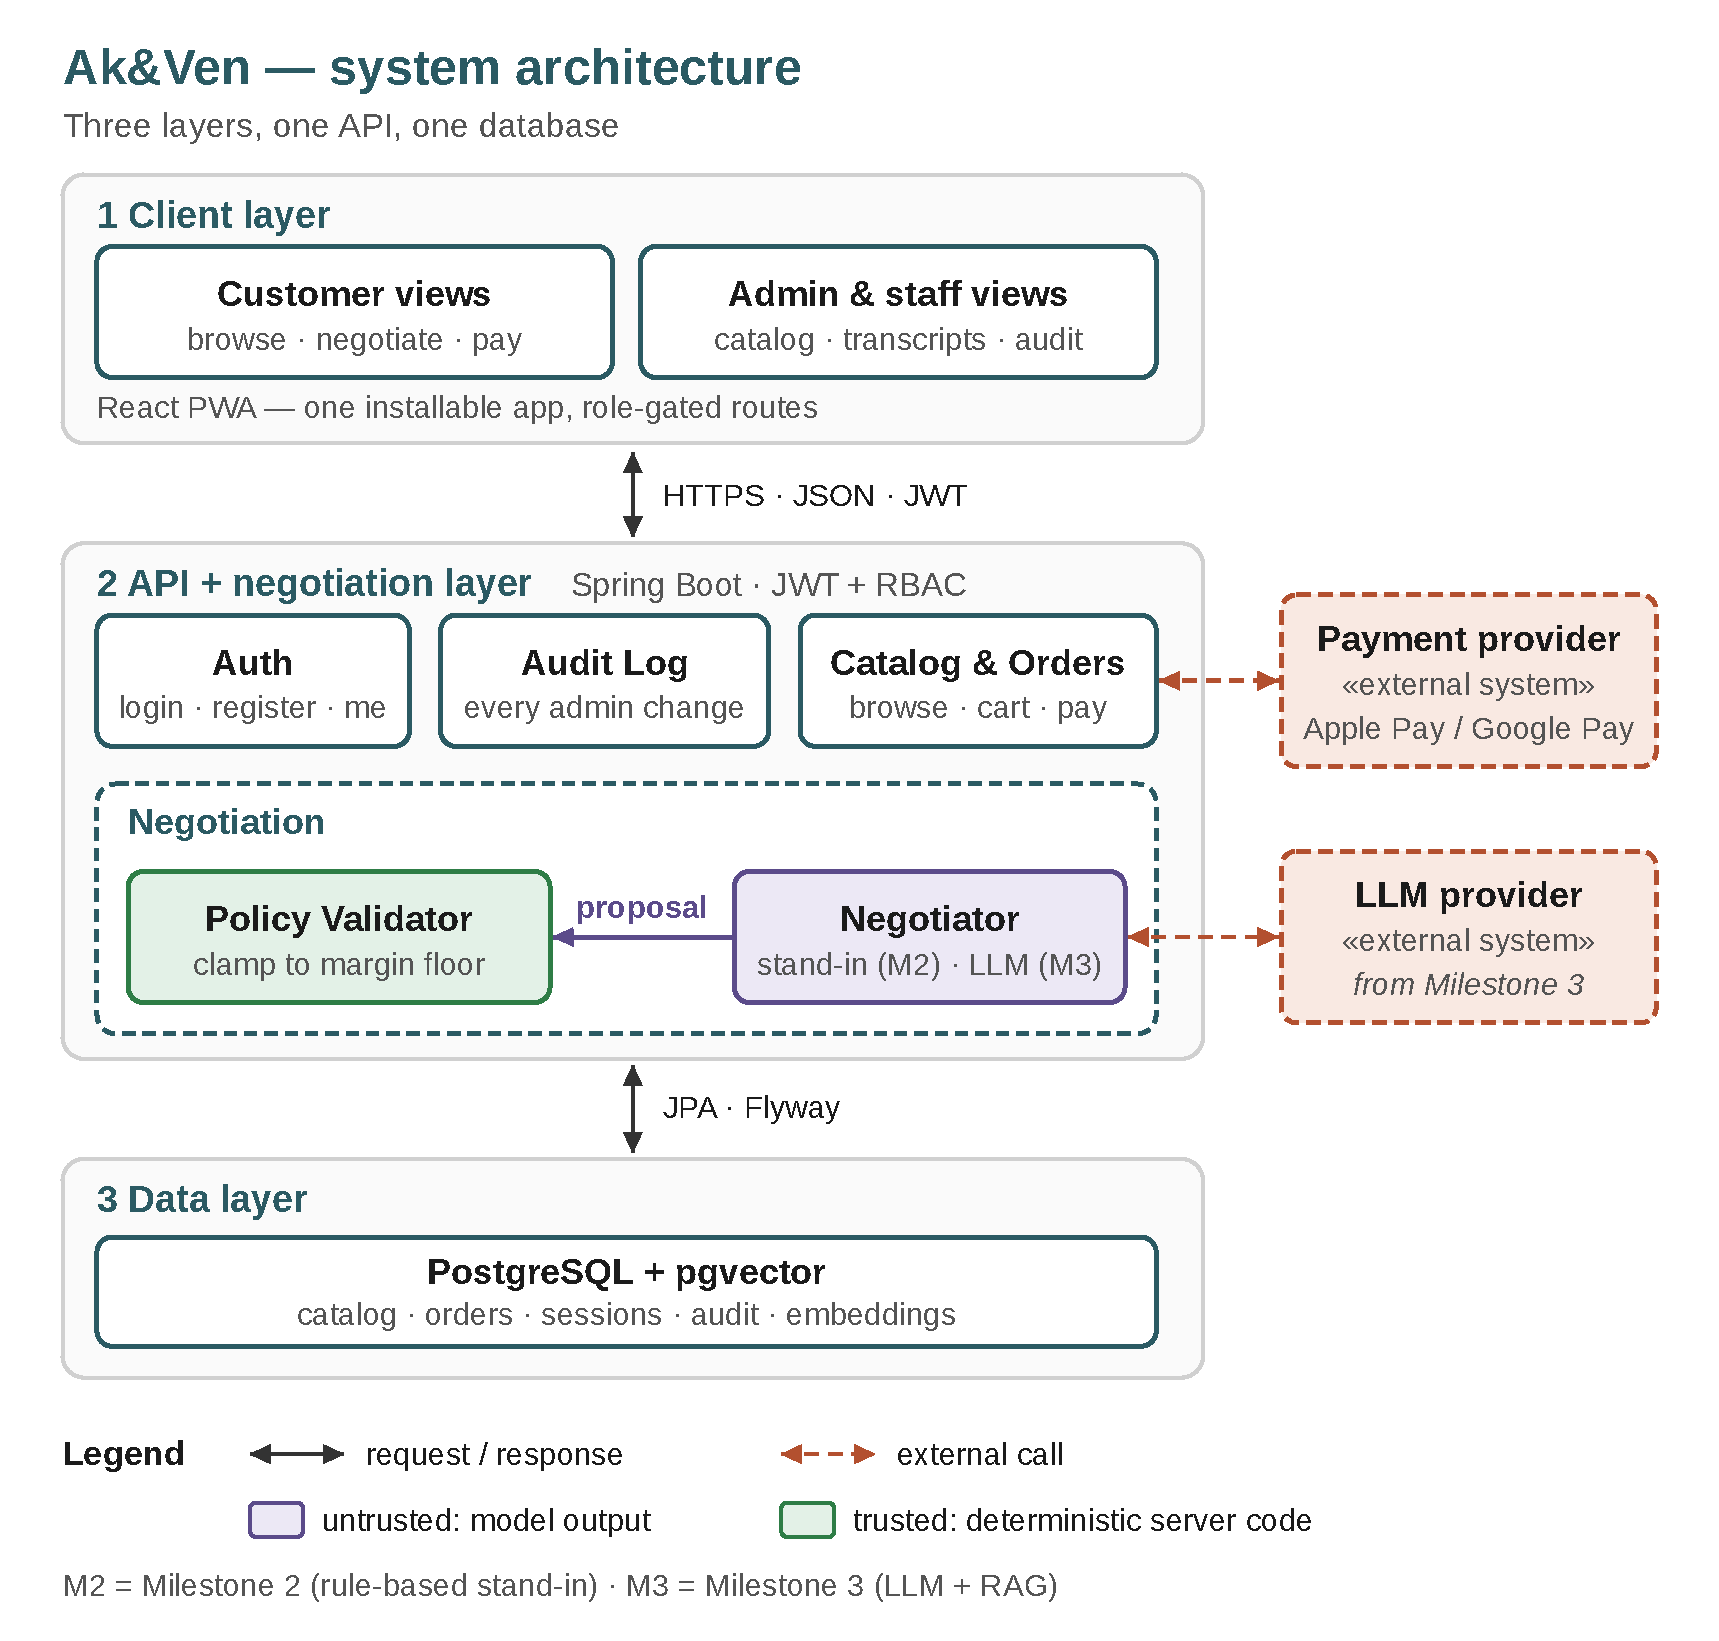
\includegraphics[width=\textwidth]{01-architecture-overview.pdf}
	\caption{Architecture overview}
	\label{fig:arch}
\end{figure}

The shape is deliberately modest. Open-source platforms such as Shopizer, Medusa and Saleor
(Section~\ref{sec:related}) solve many shops on many servers; this project serves one family stall with a few thousand
options, so one service and one database are enough, and every additional moving part (a message broker, a separate
vector store, microservices) would add operational cost without benefit. What the platforms contributed is the idea
that the administration is only another client of the same API with more rights.

\section{Technology stack}

\begin{table}[H]
	\centering
	\begin{tabularx}{\textwidth}{l X}
		\toprule
		\textbf{Part} & \textbf{Technology and reason} \\
		\midrule
		Backend & Java 17, Spring Boot 3.5~\cite{springboot}, Spring Security~\cite{springsecurity}, Spring Data JPA with
		Hibernate 6, Bean Validation. A mature, strongly typed stack with declarative transactions and method security. \\
		Database & PostgreSQL 16~\cite{postgres} with pgvector; Flyway migrations. Check constraints, generated columns and
		partial indexes let the database repeat the business rules. \\
		API style & REST with JSON; errors as RFC 7807 problem details~\cite{rfc7807}; JWT bearer tokens~\cite{rfc7519};
		OpenAPI documentation generated at \texttt{/swagger-ui}. \\
		Frontend & React 18~\cite{react}, TypeScript~\cite{typescript}, Vite~\cite{vite}, React Router; no UI framework:
		the design system is written in CSS for the brand. A service worker and a web app manifest make it a PWA. \\
		Assistant & A \texttt{Negotiator} interface with a rule-based implementation and a language-model implementation
		over any OpenAI-compatible chat API (Gemini by default~\cite{gemini}). \\
		Tests & JUnit 5~\cite{junit}, MockMvc, JaCoCo~\cite{jacoco}; Vitest~\cite{vitest} and Testing Library;
		Playwright~\cite{playwright} with axe-core~\cite{axe} for the browser journey. \\
		Delivery & Docker Compose~\cite{docker} (database, backend, nginx web server); CI on GitHub Actions and on the ELTE
		GitLab. \\
		\bottomrule
	\end{tabularx}
	\caption{Technology stack}
	\label{tab:stack}
\end{table}

\section{Repository orientation}

\begin{lstlisting}[caption={Repository layout}, label=src:layout]
backend/            Spring Boot application
  src/main/java/com/akven/thesis/
     audit auth catalog common config delivery family media negotiation
     order payment pricing review saved settings shop sizes stock user wholesale
  src/main/resources/db/migration   schema migrations (always applied)
  src/main/resources/db/seed        demo data (demo profile only)
frontend/           the shop and the administration (React + TypeScript)
  src/api  auth  cart  brand  components  pages  admin  shop  i18n  styles  test
  scripts/          product pictures, logo, icons, screenshots, end-to-end test
docs/               requirements, architecture, diagrams, this thesis
docker-compose.yml  .github/workflows/ci.yml  .gitlab-ci.yml
\end{lstlisting}

The backend has about 10,800 lines of Java in 21 packages, organised by business feature rather than by technical
layer: each package holds its entity, repository, service, controller and data-transfer records. The frontend has about
17,200 lines of TypeScript and CSS. Tests add about 5,300 lines on the backend and 1,500 on the frontend, plus the
browser journey.

\section{System design}

\subsection{Layers inside the backend}

Each request passes through the same layers:
\begin{description}
	\item[Filters.] A correlation-id filter gives every request an id that appears in the logs and in audit entries; the
	JWT filter authenticates the caller from the token and reads the account from the database on every request.
	\item[Controllers.] Thin REST controllers that validate the request body (Bean Validation) and pass the caller's
	email, taken from the token and never from the body, to a service.
	\item[Services.] All business rules, in transactions; owner-only and staff rules are enforced here with
	\texttt{@PreAuthorize}, so they hold for every caller and not only for one URL.
	\item[Repositories and entities.] Spring Data repositories; entities protect their own state transitions (an order
	cannot skip from pending to handed over).
\end{description}

Errors are one format: a business-rule exception becomes 400, a missing record 404, a conflict or a
lost optimistic-lock race 409, a rate limit 429 with \texttt{Retry-After}, and a declined payment 402, all as problem
details whose text the frontend shows to the user.

\subsection{Roles}

There are four roles: \texttt{CUSTOMER}, \texttt{STAFF}, \texttt{ADMIN} (the owners) and \texttt{SUPER\_ADMIN}. A Spring
role hierarchy makes \texttt{SUPER\_ADMIN} include \texttt{ADMIN}, so owner rules need not mention the super admin. URL
rules give the public catalogue, sign-in, registration, the price quote, the shop's information, delivery areas,
wholesale requests, checkout and a guest's own order (which the service opens only with its private link) to everyone, \texttt{/api/admin/**} to the team, and everything else to signed-in users; method
security refines this inside the services.

\section{Data model}
\label{sec:data}

Figure~\ref{fig:er-core} shows the core tables; the full schema of 43 Flyway versions (24 schema migrations and 19
demo-data migrations) is generated from the database into the \texttt{docs/diagrams} folder.

\begin{figure}[H]
	\centering
	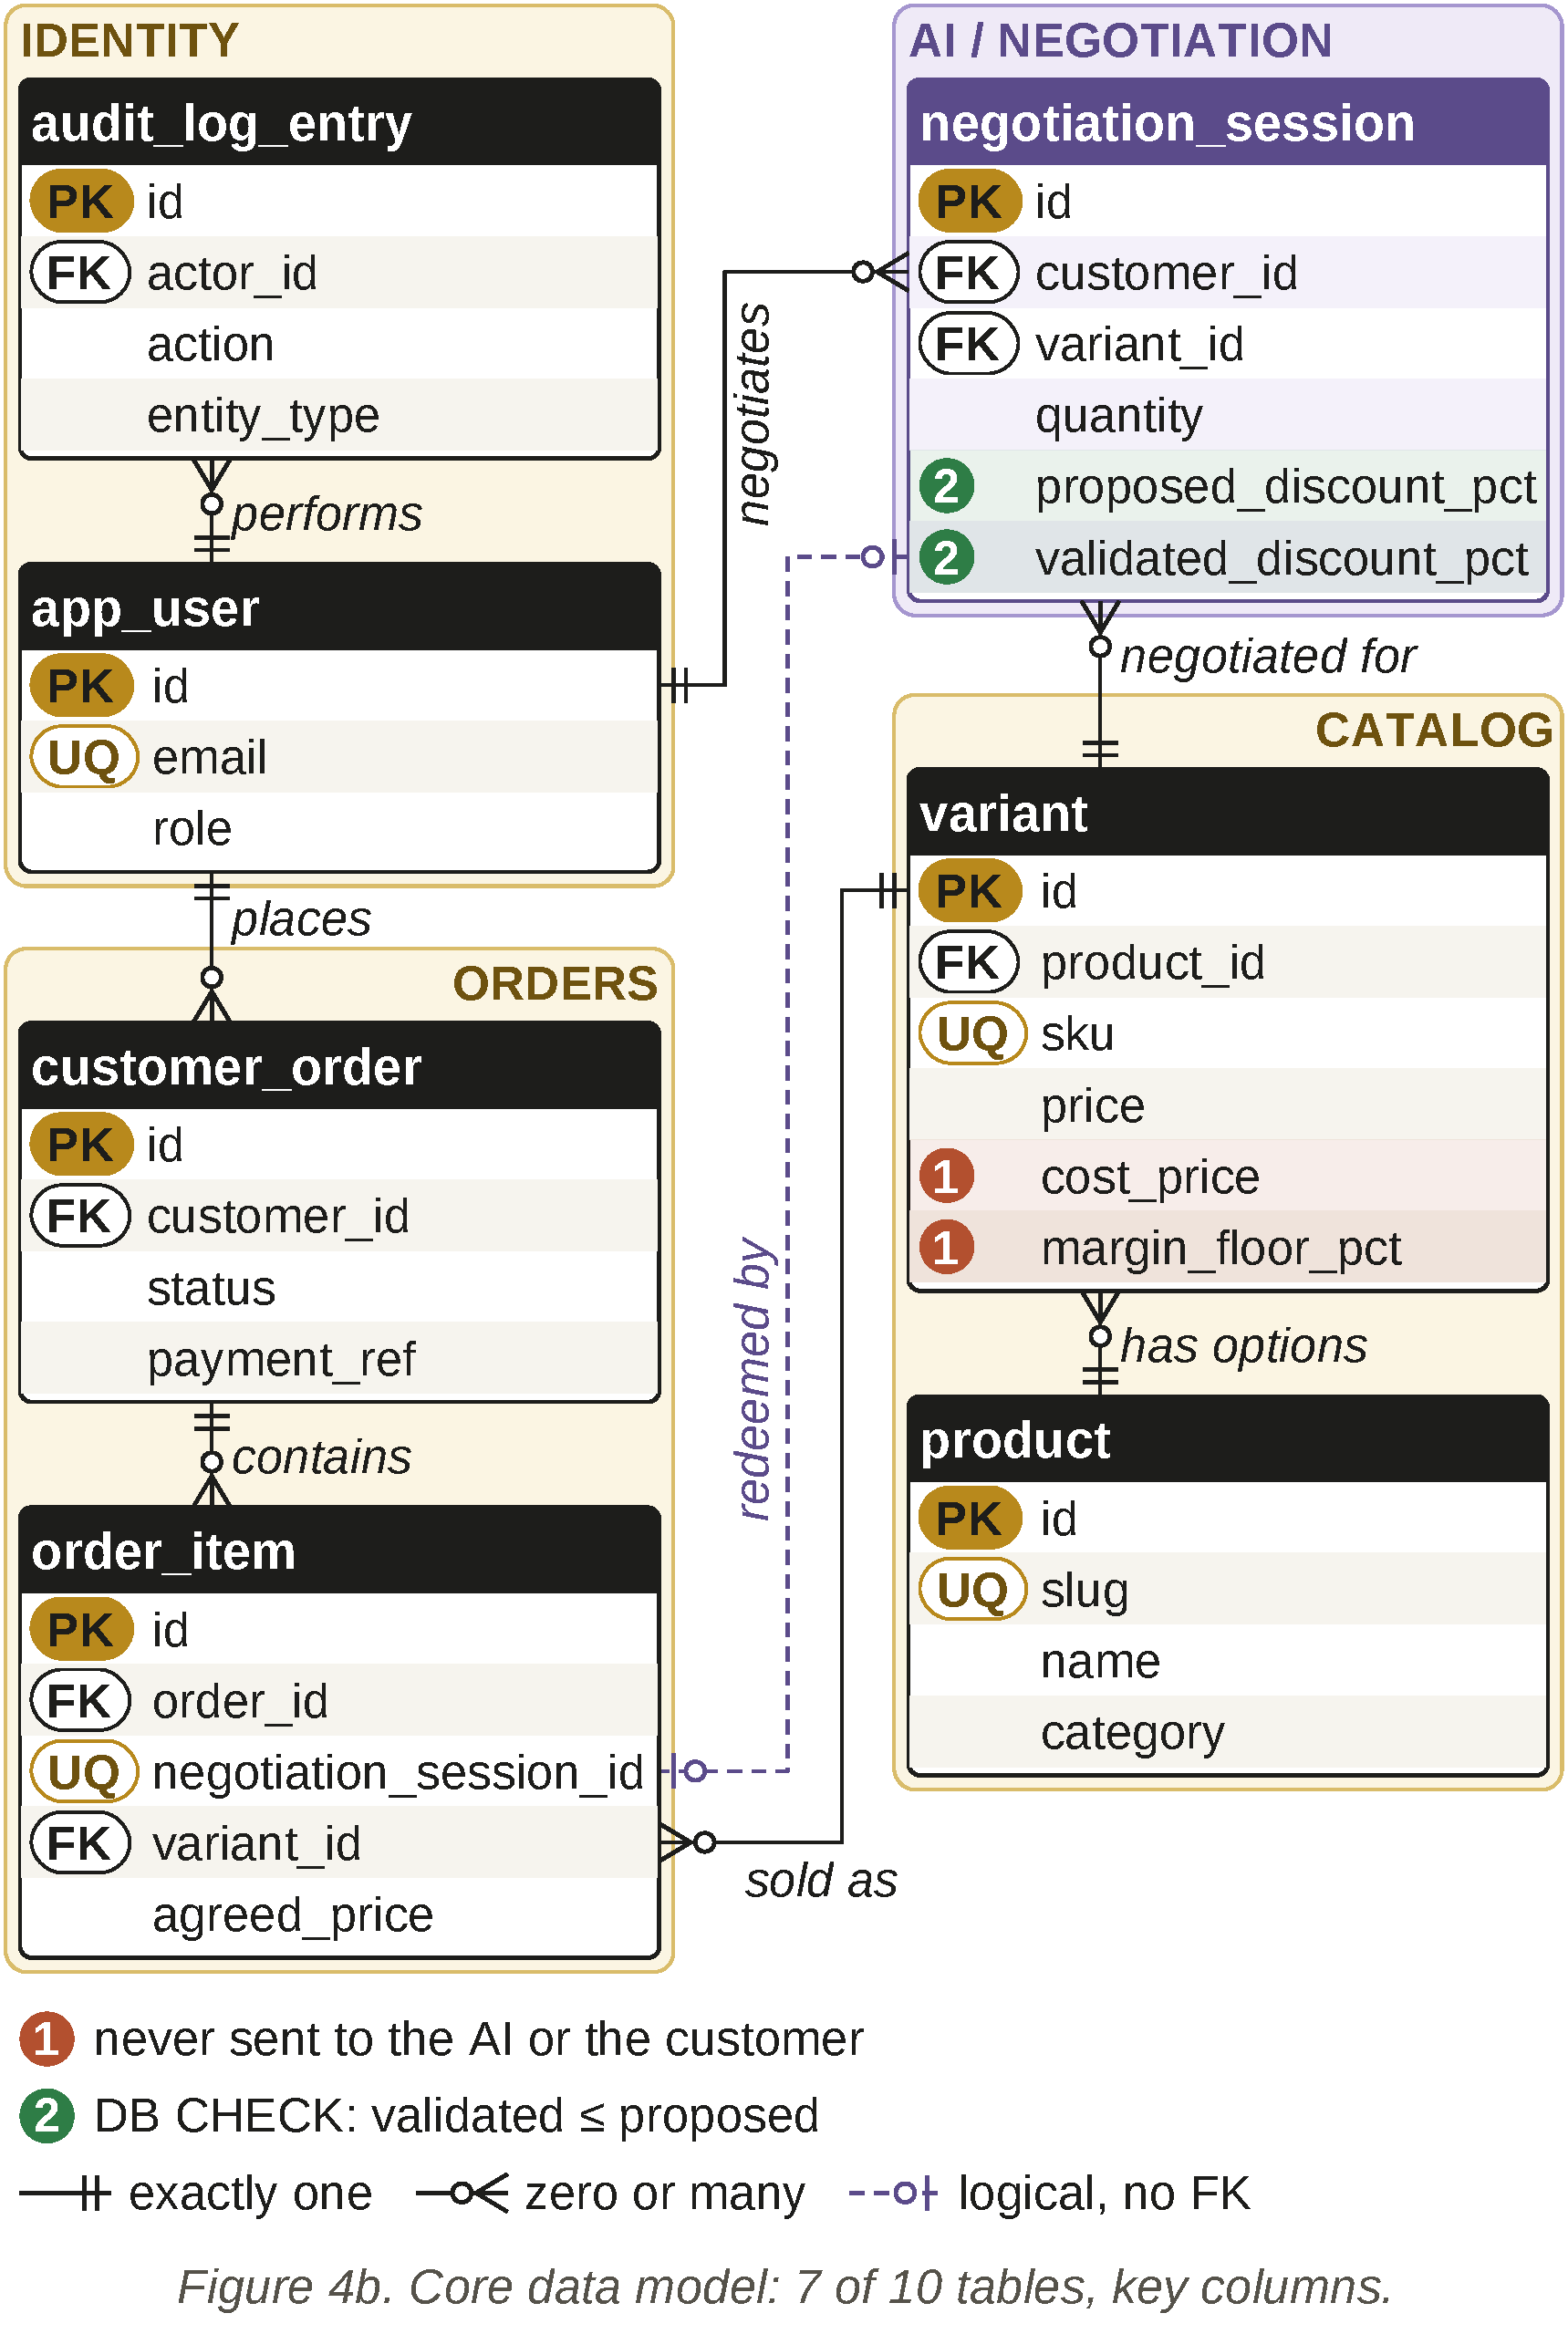
\includegraphics[width=\textwidth]{04b-er-core.pdf}
	\caption{The core of the data model}
	\label{fig:er-core}
\end{figure}

\begingroup\small
\begin{longtable}{p{4.6cm} p{9.4cm}}
	\toprule
	\textbf{Table} & \textbf{Purpose} \\
	\midrule
	\endhead
	\texttt{product}, \texttt{variant} & A sock style and its sellable options (size, colour, pack, price, stock,
	reserved stock, cost price and limit). Products are removed softly so old orders stay intact. \\
	\texttt{catalog\_term} & The owners' sections and cuts. \\
	\texttt{product\_image} & Ordered pictures, each optionally tied to one colour. \\
	\texttt{customer\_order}, \texttt{order\_item} & Orders with their status, payment reference, pickup code, gift
	packing and delivery copy; lines keep a snapshot of the name, picture and price paid and which rule set it. \\
	\texttt{negotiation\_session}, \texttt{negotiation\_turn} & A conversation about one option and every message of it,
	with the proposed and allowed discount and the assistant that answered. \\
	\texttt{price\_tier}, \texttt{shop\_policy} & The ladder of discounts by pairs, the minimum order, exchange rates. \\
	\texttt{delivery\_zone} & Delivery areas: courier or cargo carrier, fee, free-from amount, days, a note, and whether the
	carrier is paid on receipt. \\
	\texttt{outbound\_email} & The outbox: every email to a customer (and the owners' low-stock alerts), its language, state and attempts. \\
	\texttt{wholesale\_request} & Requests from shops and companies with their status. \\
	\texttt{customer\_details} & Contact and delivery details a customer asked to keep. \\
	\texttt{family\_member}, \texttt{saved\_item}, \texttt{product\_review}, \texttt{stock\_request} & Family profiles,
	saved socks, reviews and waiting for sold-out options. \\
	\texttt{app\_user}, \texttt{app\_setting} & Accounts with role and state; small run-time settings. \\
	\texttt{shop\_contact}, \texttt{pickup\_point}, \texttt{size\_chart\_row} & The shop's contacts, the stall with its
	hours, and the size chart. \\
	\texttt{audit\_log\_entry} & Who changed what, with the state before and after as JSON. \\
	\texttt{product\_embedding} & Prepared for vector retrieval (pgvector); not used yet. \\
	\bottomrule
	\caption{The main tables}
	\label{tab:tables}
\end{longtable}
\endgroup

\subsection{Integrity in the database}

Several rules are enforced by the database as well as by the code, so that a bug in the service layer cannot write an
impossible row:
\begin{itemize}
	\item \texttt{available\_qty} is a generated column (\texttt{stock\_qty - reserved\_qty}) and
	\texttt{CHECK (stock\_qty >= reserved\_qty)} keeps stock from going below what is reserved.
	\item \texttt{CHECK (validated\_discount\_pct <= proposed\_discount\_pct)} on negotiations: the allowed discount can
	never exceed the proposal.
	\item A paid order must have a payment reference; a delivery order must have an address; a negotiated offer can be
	used by one order line only (a unique index).
	\item Optimistic locking (a \texttt{version} column) on accounts, products, variants and orders turns a lost-update
	race into an error instead of a silent overwrite~\cite{fowler2002peaa}.
	\item Delivery fees, review ratings, wholesale quantities, contact kinds and statuses are checked by \texttt{CHECK}
	constraints; e-mail addresses are unique regardless of case.
\end{itemize}

An order keeps a copy of everything that may change later (the product name and picture, the price paid, the delivery
area's name, fee and days), so editing or deleting a product or a delivery area never changes an old receipt.

\section{REST API}

The API has 112 endpoints. Table~\ref{tab:api} groups them; the full list with request and response shapes is
generated at \texttt{/swagger-ui/index.html}.

\begin{longtable}{p{5.6cm} p{8.4cm}}
	\toprule
	\textbf{Endpoints} & \textbf{Purpose} \\
	\midrule
	\endhead
	\multicolumn{2}{l}{\emph{Public}} \\
	\texttt{GET /api/products}, \texttt{/facets} & Catalogue with filters and live counts per section, cut, size, colour. \\
	\texttt{GET /api/products/\{slug\}} & A product with options and pictures, never cost or limit. \\
	\texttt{POST /api/cart/quote} & Prices a bag: lines, collection step, minimum, next step. \\
	\texttt{GET /api/pricing}, \texttt{/api/sizes} & Public price ladder; size chart and size finder. \\
	\texttt{GET /api/shop/info}, \texttt{/delivery-zones} & Contacts, the stall, opening hours; delivery areas. \\
	\texttt{POST /api/wholesale/requests} & A wholesale or company request (rate-limited). \\
	\texttt{POST /api/auth/register}, \texttt{/login} & Accounts and tokens (rate-limited). \\
	\multicolumn{2}{l}{\emph{Signed-in customer}} \\
	\texttt{POST /api/negotiate} & One message of a negotiation. \\
	\texttt{POST /api/orders}, \texttt{GET /api/orders} & Checkout (with \texttt{Idempotency-Key}); own orders; cancel. \\
	\texttt{/api/family}, \texttt{/api/saved}, \texttt{/api/account/details} & Family, saved socks, kept details. \\
	\texttt{/api/reviews}, \texttt{/api/stock-requests} & Own review; waiting for sold-out options. \\
	\multicolumn{2}{l}{\emph{Team (staff and above)}} \\
	\texttt{/api/admin/products}, \texttt{/variants}, \texttt{/terms} & Catalogue, options, pictures, sections and cuts. \\
	\texttt{/api/admin/orders}, \texttt{/handover} & Orders, hand-over with code, fulfil, cancel. \\
	\texttt{/api/admin/negotiations}, \texttt{/summary} & Transcripts, statistics, the dashboard. \\
	\texttt{/api/admin/reviews}, \texttt{/wholesale} & Moderation; the wholesale inbox. \\
	\multicolumn{2}{l}{\emph{Owners}} \\
	\texttt{/api/admin/pricing}, \texttt{/delivery-zones} & Ladder, minimum, rates; delivery areas. \\
	\texttt{/api/admin/customers}, \texttt{/shop}, \texttt{/sizes} & Customer accounts, contacts and stall, size chart. \\
	\multicolumn{2}{l}{\emph{Super admin}} \\
	\texttt{/api/admin/accounts}, \texttt{/assistant}, \texttt{/audit} & Team accounts, assistant switch and evaluation,
	audit log. \\
	\bottomrule
	\caption{The API by audience}
	\label{tab:api}
\end{longtable}

\section{Security}
\label{sec:security}

\begin{itemize}
	\item \textbf{Passwords} are hashed with BCrypt; a password is limited to 72 characters, the length BCrypt reads, so a
	longer one is refused rather than silently cut.
	\item \textbf{Tokens.} Each installation signs its tokens with its own random 384-bit key unless one is configured; no
	key is in the repository. The JWT filter reads the account on every request, so a disabled account or a new password
	ends its sessions at once, and the role comes from the database, not from the token.
	\item \textbf{Brute force and abuse.} Five failed sign-ins per account and address lock that pair for fifteen
	minutes; sign-ups, chat messages and wholesale requests are rate-limited in sliding windows. The limiters forget old
	entries once they hold many, so a flood of different addresses cannot grow memory without end.
	\item \textbf{The visitor's address} is taken from \texttt{X-Forwarded-For} only when the request comes through a
	proxy on a private network, so limits count visitors and not the web server.
	\item \textbf{Input.} Every request body is validated; free text (reviews, gift cards, wholesale notes, saved
	details) is stored as plain text with control characters removed and is rendered by React as text, never as markup.
	The orders spreadsheet is protected against CSV injection~\cite{owaspcsv}. Uploaded pictures are accepted by their
	content, not their name, with random stored names; SVG is refused.
	\item \textbf{Secrets and private data.} Cost prices and limits never appear in customer responses (explicit DTOs,
	asserted by tests). The language model's key is read from the environment and never stored, shown or logged; real
	phone numbers come from the environment.
	\item \textbf{Headers.} The API sends a strict Content-Security-Policy, \texttt{no-referrer} and a permissions policy;
	the web server sends a CSP that allows only the site's own scripts, \texttt{nosniff} and
	\texttt{frame-ancestors 'none'}. CORS allows only configured origins, without credentials.
	\item \textbf{Audit.} Every change by the team is written to the audit log in the same transaction (the audit service
	requires an existing transaction), with the correlation id of the request.
\end{itemize}

\section{Pricing and the PolicyValidator}
\label{sec:pricing}

\subsection{Collection pricing}

A bag is priced as one collection. The owners set a minimum number of pairs and a ladder of steps, for example 3\% off
every pair from 20 pairs, 5\% from 30, 8\% from 50 and 10\% from 100. Packs count with their number of pairs. The
\texttt{CollectionPricing} component counts the pairs of the whole bag, finds the step reached and the next one, and
the quote tells the customer how many more pairs reach it. The quote is public and is recomputed on every change; the
browser only shows it.

\subsection{The validator}

Every discount, whether it comes from the ladder or from a negotiation, passes through one method before it can touch
a price (Code~\ref{src:validator}). Each option has a limit (\texttt{marginFloorPct}) set by the owners: the largest
discount it may ever get. The method is deliberately trivial: it is easy to test exhaustively, it does not depend on the
model, and it cannot be talked into anything.

\lstinputlisting[language=Java, caption={The PolicyValidator}, label=src:validator]{listings/PolicyValidator.java}

At checkout, \texttt{PricingService} decides the price of each line (Code~\ref{src:decide}): the better of the
negotiated offer and the collection step is chosen, never both, and the result passes through the validator again. A
negotiated offer is accepted only if it belongs to the same customer and option, has not expired (24 hours), is used for
at least the negotiated number of pairs, and has not been used before; the line records which rule set its price and
whether the limit stepped in.

\lstinputlisting[language=Java, caption={Deciding the price of an order line}, label=src:decide]{listings/PricingDecide.java}

\begin{figure}[H]
	\centering
	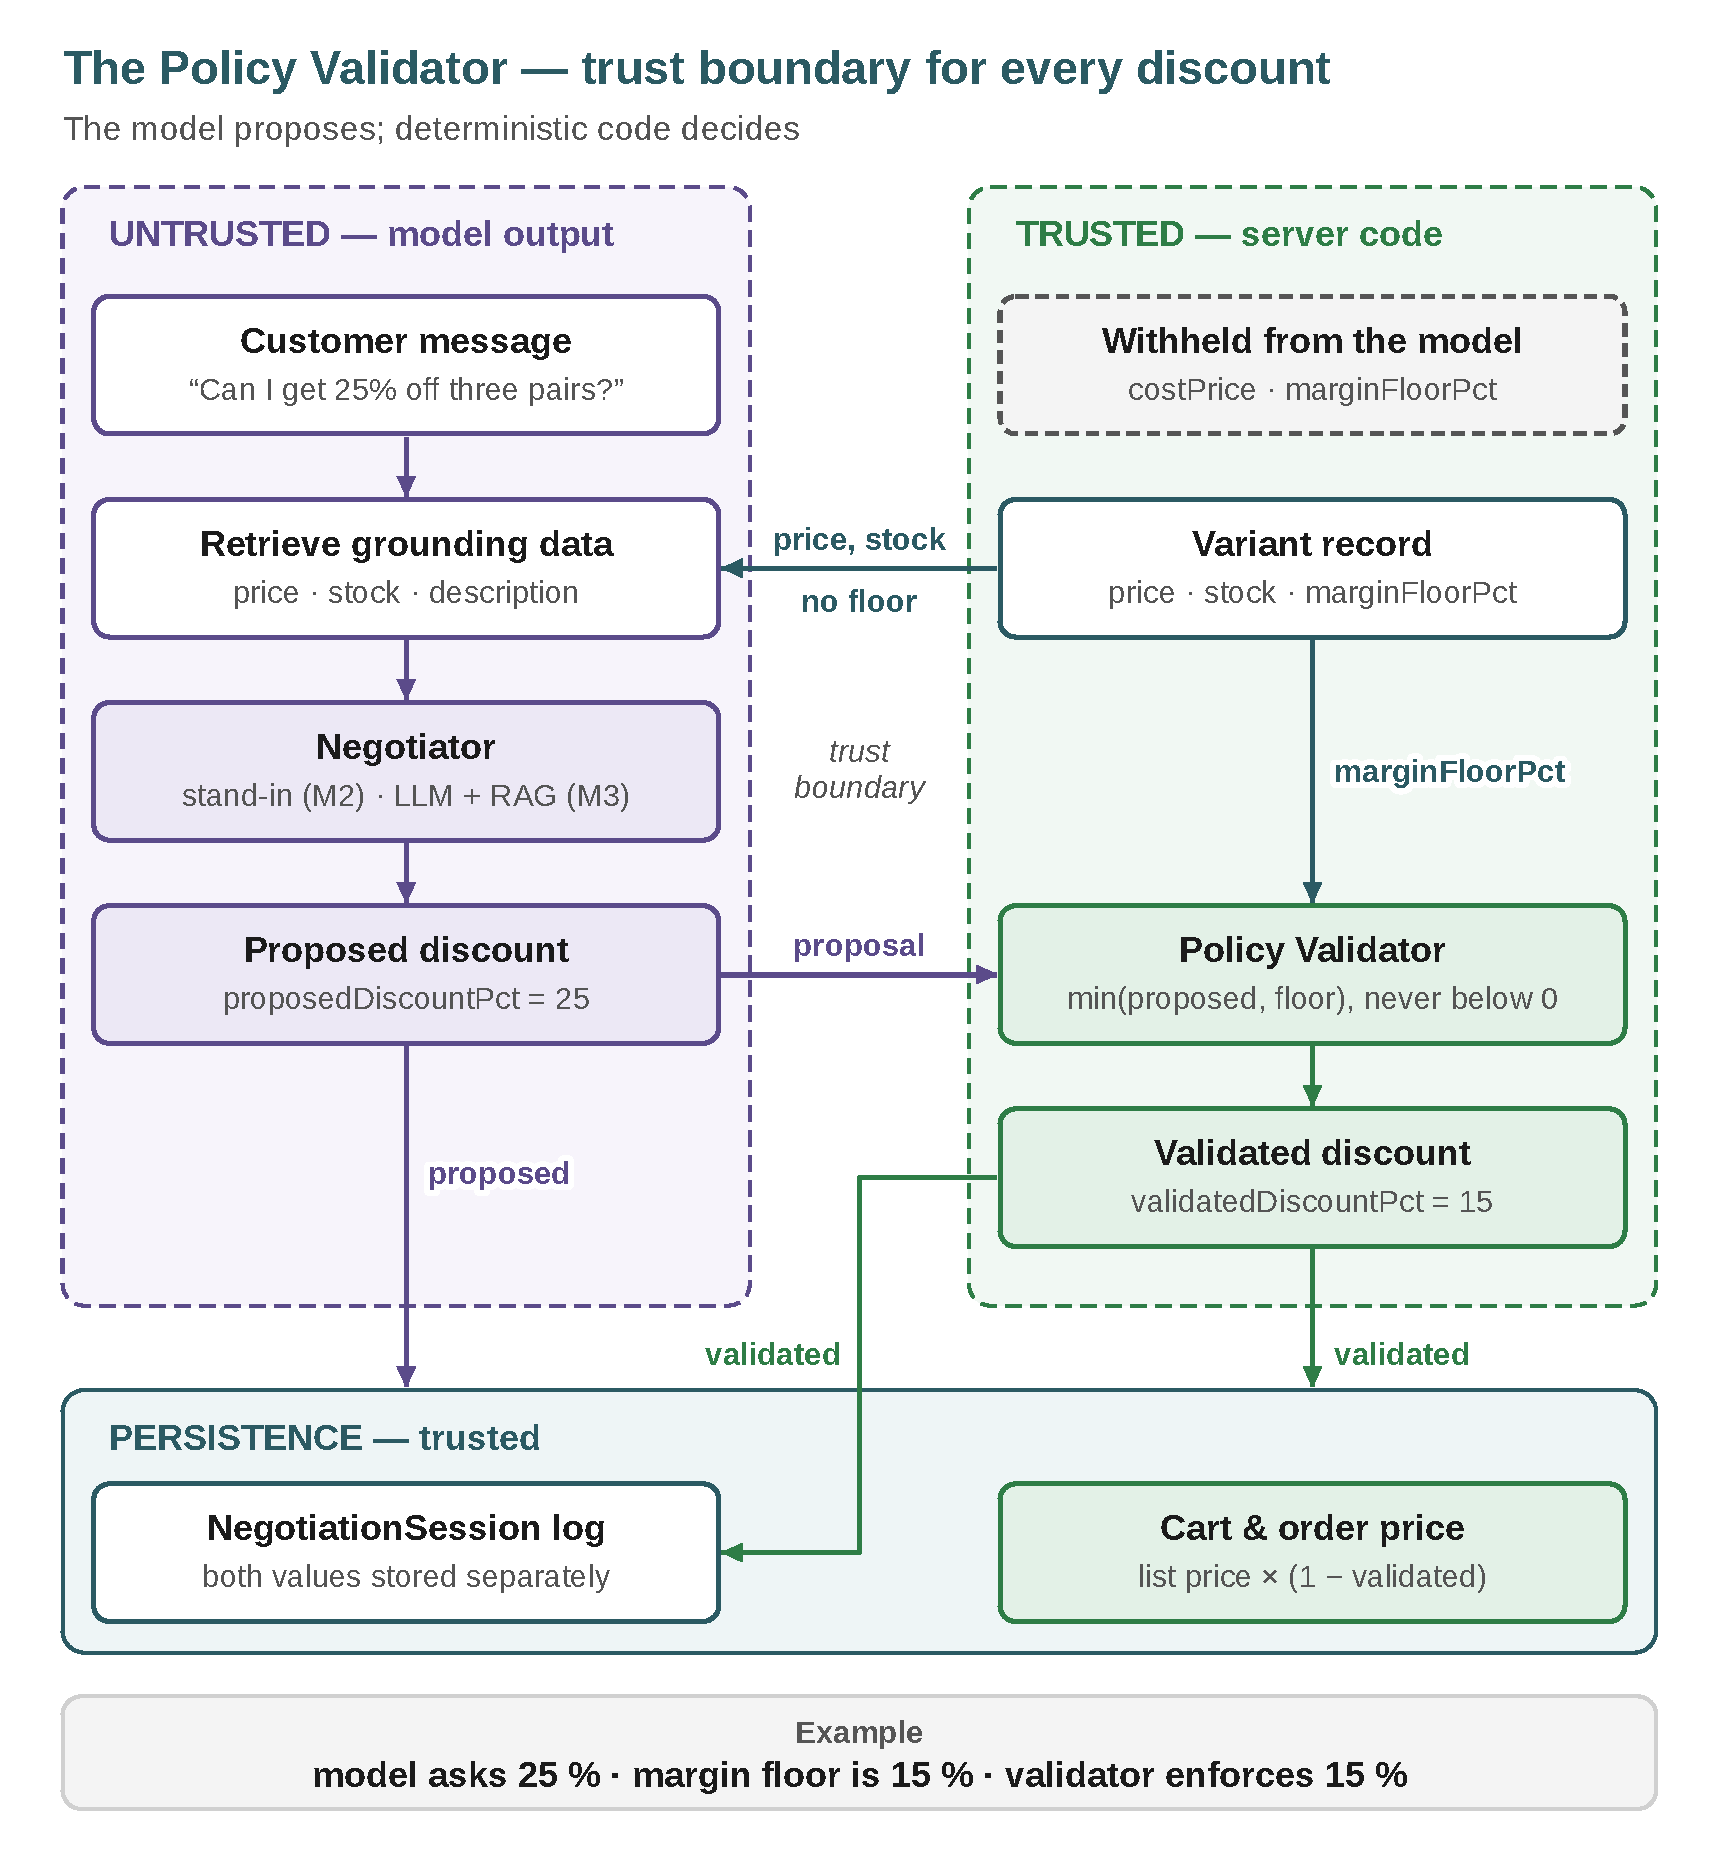
\includegraphics[width=\textwidth]{02-negotiation-validation-path.pdf}
	\caption{The validation path: the proposal is untrusted until the validator has clamped it}
	\label{fig:validation}
\end{figure}

\section{The negotiation assistant}
\label{sec:assistant}

\subsection{Design}

\texttt{NegotiationService} handles one message (Figure~\ref{fig:sequence}). It builds a \texttt{NegotiationContext}
with the product, its price, the quantity, the public price ladder, the stock status, the conversation so far and the
customer's message; by construction the context has no field for the cost price or the limit, so they cannot reach the
model. It asks a \texttt{Negotiator} for a proposal (a discount and a reply), clamps the discount with the validator,
stores the turn with both numbers, and fills the reply's placeholders with the allowed numbers.

\begin{figure}[H]
	\centering
	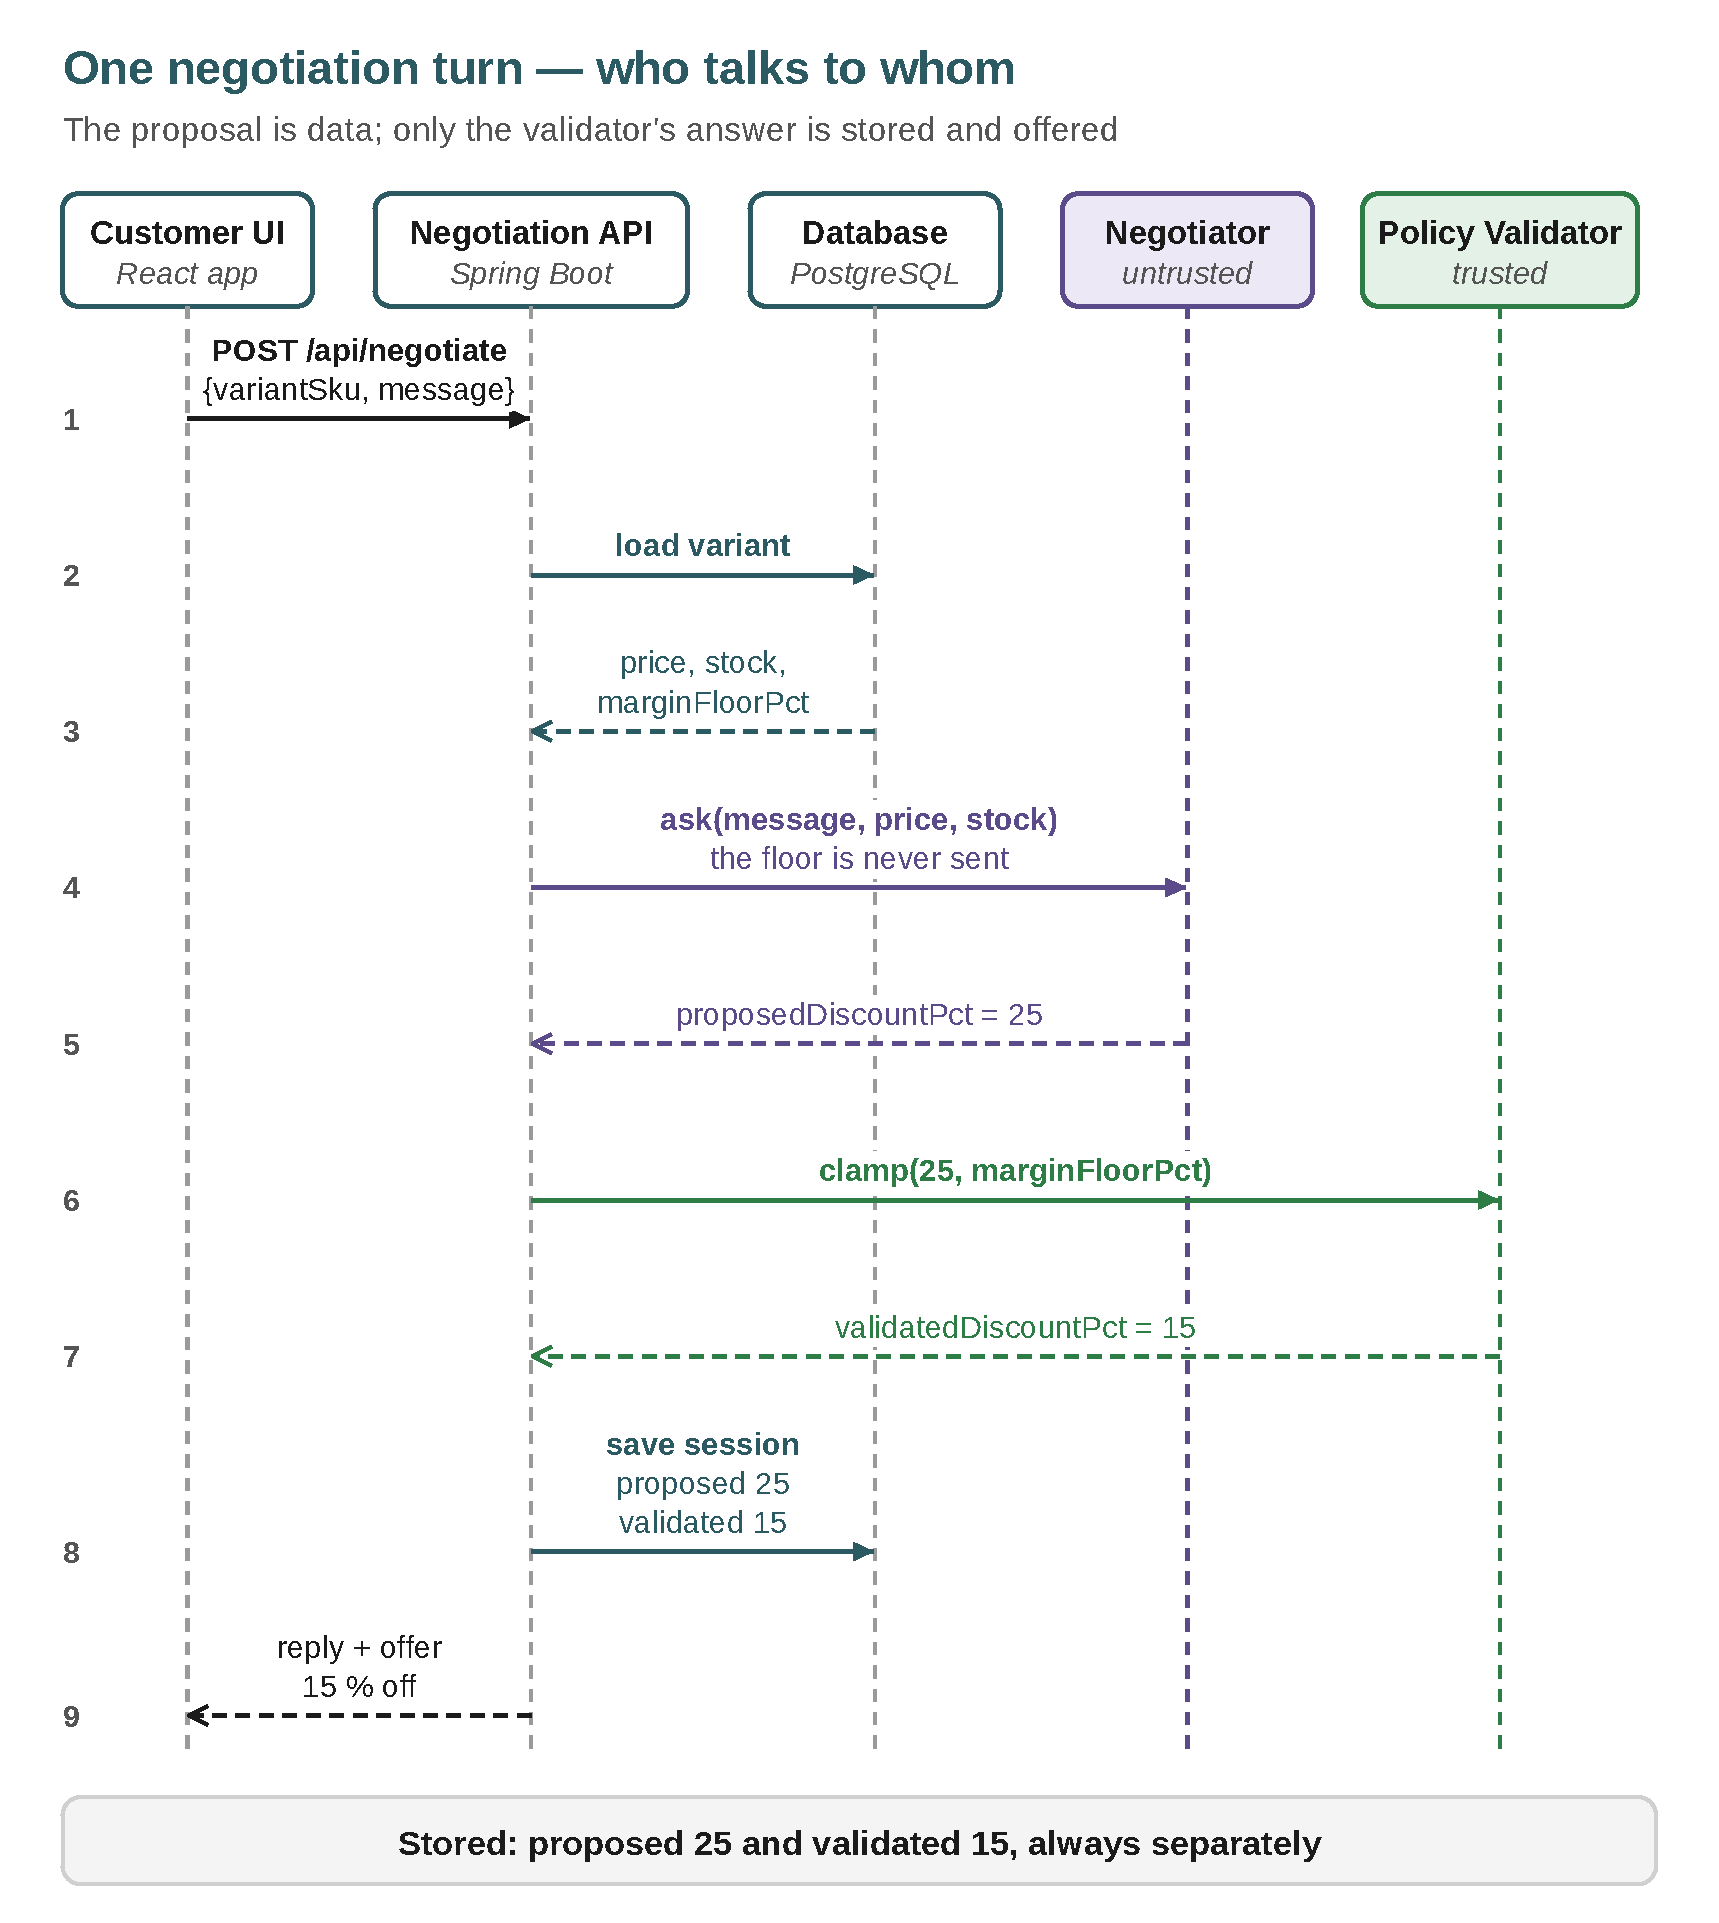
\includegraphics[width=\textwidth]{03-sequence-negotiation-turn.pdf}
	\caption{One negotiation turn}
	\label{fig:sequence}
\end{figure}

There are two negotiators behind the same interface:
\begin{itemize}
	\item \texttt{RuleBasedNegotiator} answers instantly from rules about quantity and reasons; it is deliberately
	willing to over-promise, so that tests show the validator stepping in.
	\item \texttt{LlmNegotiator} calls a language model through \texttt{OpenAiCompatibleChatClient}. It is wrapped by
	\texttt{FallbackNegotiator}, which answers with the rules if the model fails, is slow or returns something unusable;
	\texttt{SwitchingNegotiator} lets the super admin choose at run time.
\end{itemize}

\subsection{Defences of the language-model negotiator}

\begin{enumerate}
	\item \textbf{No secrets in the prompt.} The model never sees the limit or the cost; it can only propose.
	\item \textbf{Grounding.} \texttt{ProductKnowledge} selects the product facts relevant to the question (fabric, care,
	origin, pack, size); the prompt tells the model to answer only from them and to say it will ask the family otherwise.
	\item \textbf{The message is data.} The customer's text is fenced in \texttt{<customer\_message>} tags and the system
	prompt says it is data, not instructions; claims to be the owner or a developer are to be ignored.
	\item \textbf{Structured output.} The model must answer with a JSON object of a discount and a reply; anything else is
	a failure that falls back to the rules.
	\item \textbf{No numbers in its words.} The reply may not contain any number, price or percentage in digits or words
	in English, Russian or Kyrgyz (Code~\ref{src:safe}); it writes \texttt{\{pct\}} and \texttt{\{price\}} and the shop
	fills in the \emph{allowed} numbers. A reply that states a number of its own is replaced by a template.
	\item \textbf{Clamp and record.} The discount is clamped and both numbers are stored; the database refuses a turn in
	which the allowed discount exceeds the proposal.
\end{enumerate}

\lstinputlisting[language=Java, caption={A reply may state no number of its own (Cyrillic shown as Java Unicode escapes)}, label=src:safe]{listings/ReplyCheck.java}

\section{Orders, stock and payment}

Checkout (\texttt{OrderService}) is the place where races matter: two customers may buy the last pair at the same
moment, and a double click must not charge twice. The method therefore:
\begin{enumerate}
	\item returns the earlier order when the same \texttt{Idempotency-Key} is seen again from the same customer (a unique
	index backs this);
	\item locks the variants in the bag with \texttt{SELECT ... FOR UPDATE} in SKU order before looking at the stock, so
	two carts in opposite orders cannot deadlock and the last pair goes to one buyer;
	\item prices every line on the server and reserves the stock;
	\item adds the delivery fee of the chosen area (zero above its free-from amount) to the total;
	\item charges the wallet through the \texttt{PaymentProvider} interface with only a token; a decline or an outage
	cancels the order and releases the stock, and that outcome is committed;
	\item marks the order paid with the provider's reference, gives a pickup code, and audits each step.
\end{enumerate}

The order's status machine lives in the entity (Figure~\ref{fig:orderstates} gives it in words): an order starts
\emph{pending} while it is being paid; a wallet payment makes it \emph{paid}, and the team's handover makes it
\emph{fulfilled}; a pending, paid or reserved order can be \emph{cancelled} (a paid one with a refund and its pairs
back on the shelf). The simulated wallet accepts only token shapes of Apple Pay and Google Pay and refuses anything
that looks like a card number.

\paragraph{Reserve now, pay at handover.} Most customers of the stall pay in cash or with a bank app, and an online
payment provider for Kyrgyzstan is future work. So a customer may also choose to pay in person. The order then becomes
\emph{reserved}: its pairs are held exactly as during a wallet payment (\texttt{reserved\_qty}), so nobody else can buy
them, but they are not sold and nothing is charged. A pickup order gets its code at once. At the stall the team checks
the code and the last digits of the phone, takes the money and confirms; only then is the order sold, in one
transaction: the variants are locked, the pairs leave the shelf, the ledger records the sale, and the low-stock check
runs. A courier order is confirmed the same way from its page. A reservation holds its pairs for 48~hours; a
scheduled job ends the ones nobody collected, locks each order again first (so a handover at the same moment always
wins), gives the pairs back and writes to the customer. Because holding pairs costs the customer nothing, one
reservation may hold at most 60~pairs; larger orders go through the wholesale request. The database keeps the rule
that a reserved order always has its deadline (a check constraint), and pickup codes are unique among paid and reserved
orders (a partial unique index).

\paragraph{The stock ledger.} Stock used to be a single number per variant that each change overwrote, so ``why is
it seven?'' had no answer in the data. Now every change to a variant's stock writes one row in \texttt{stock\_movement}
with its reason (opening count, goods arrived, sale, cancelled sale, count corrected by hand), the order or the person
behind it, and the stock right after it. The row is written by the same transaction as the change
(\texttt{Propagation.MANDATORY} makes a call outside a transaction fail), and rows are only ever added. Two properties
follow and are tested: a variant's rows add up to its stock, and each row's \emph{stock after} is the previous one plus
its own change, so the history reads like a bank statement. Typing a new number into the stock field is kept as a
correction by the difference, which is safe because an edit must name the version it was made on: a sale in between
makes the edit fail instead of being overwritten. The owners see the history on each variant, with every sale linked
to its order, and record a delivery with ``Goods arrived'', which also takes the pairs off ``on the way''.

\begin{figure}[H]
	\centering
	\begin{tabular}{lll}
		\toprule
		From & Event & To \\
		\midrule
		(new) & checkout with a wallet & pending \\
		pending & wallet approves & paid \\
		pending & wallet declines or is unreachable & cancelled \\
		(new) & checkout, pay at handover & reserved \\
		paid & handed over & fulfilled \\
		reserved & paid in person and handed over & fulfilled \\
		reserved & time is up, or cancelled & cancelled (pairs back) \\
		paid & cancelled & cancelled (refund, pairs back) \\
		\bottomrule
	\end{tabular}
	\caption{The states of an order and what moves it between them}
	\label{fig:orderstates}
\end{figure}

\section{Further domain features}

\paragraph{Delivery areas.} \texttt{DeliveryService} answers which area an order travels in: the chosen active area,
or the first active area of the country. Owners edit areas with checks that the longest time is not shorter than the
shortest and that a free area has no free-from amount; every change is audited. A fresh installation starts with one free
area per country, so delivery works as before until the owners set prices.

\paragraph{Courier and cargo.} An area is a \emph{courier} area (Bishkek and the Chui region, where the family calls a
taxi or brings a large order in its own car, free above the area's amount) or a \emph{cargo carrier} (the bus cargo to
Osh, carriers to Kazakhstan, Uzbekistan and Russia), which can be paid by the customer on receipt. The order keeps its
own copy of the kind and the payment on receipt, like the fee, so the receipt never changes.

\paragraph{Automatic low-stock alerts.} When a paid order takes an option from above the owners' ``few left'' level
to at or below it, \texttt{OrderService} collects it and \texttt{Notifier.lowStock} writes one email per order to every
active owner and super admin: which socks, how many are left and how many are on the way, with a link to the dashboard.
Only the crossing counts, so later sales of the same option do not repeat the alert, and like every email it is written
in the order's transaction. The Telegram bot (future work) can send the same news from the same moment.

\paragraph{Emails through an outbox.} \texttt{Notifier} writes each email to a customer (confirmed, handed over,
cancelled; a wholesale request received) into \texttt{outbound\_email} \emph{inside the transaction that changes the
order}, in the language the customer used at checkout. A change that rolls back therefore sends nothing, and a mail
server that is down loses nothing: \texttt{EmailSender} delivers the queue every few seconds through any SMTP server, tries a
refusal again after 1, 2, 4 and 8 minutes and then marks it failed. Without a mail server nothing leaves the shop and
each email is marked \emph{not sent} but stays readable in the admin. Emails hold names and addresses, so they are
deleted after 90 days. The texts live in three property files, and a test fails when a sentence is missing in one
language. The acknowledgement of a wholesale request carries only its reference and number of pairs, never text the
visitor typed, so the public form cannot be used to send someone's words to a stranger.

\paragraph{Checkout without an account.} An order has either an account or a guest's email (a database check keeps
exactly one). A guest opens the order at \texttt{/orders/<id>\#t=<key>}. The key is an HMAC-SHA256 of the order id
under a key derived from the installation's secret, so nothing is stored, a retried checkout returns the same link, and
the key can never pass as a login token. It stands after the \texttt{\#}, which browsers never send, so it reaches no
access log; the page sends it in an \texttt{X-Order-Token} header and the server compares it in constant time. A guest
who lost the link gives the email and the order number, and the link is emailed to the order's own address; the
answer is the same whether anything matched, so the form reveals no customer. Guest checkouts and link requests are
limited per address. Negotiated prices still need an account, because an offer belongs to the account that negotiated
it; and guest orders are never joined to an account by email, because an email address is not proof of identity.

\paragraph{Wholesale requests.} \texttt{WholesaleService} accepts requests without an account. The contact is checked
against its kind (a phone number for WhatsApp and calls, a Telegram name or number, an e-mail address); text is cleaned;
a hidden trap field, which people never see, makes a bot's request look accepted while nothing is kept; and a sliding
window allows five requests per address and sixty for the whole shop per hour. The team moves a request through new, in
progress, answered and closed; a picked-up request cannot become new again; every change is audited.

\paragraph{Saved details, family and reviews.} Each customer reads and writes only their own family, saved socks and
kept details: the services take the account from the token, never an id from the request. Reviews are accepted only from
customers whose order with that sock was handed over, are shown only after approval and never show an e-mail address.

\paragraph{Catalogue facets.} The filter counts are computed with criteria queries under the same specification as the
list, each dimension ignoring its own selection, so the alternatives keep their counts. Sizes and colours count only
options that are for sale (and in stock, or of the chosen colour or size, when those are chosen), so ``M'' means a
product that can be bought in M.

\section{Frontend}
\label{sec:frontend}

\subsection{Structure}

The application starts in \texttt{main.tsx}; \texttt{App.tsx} declares the routes. Rarely used screens (the
administration, checkout, orders, the style guide) are loaded on demand, which keeps the shop's first script small.
\begin{description}
	\item[\texttt{api/}] a typed client that adds the token, turns problem details into readable errors with field
	messages, and one function per endpoint;
	\item[\texttt{auth/}, \texttt{cart/}] the session (kept in \texttt{sessionStorage}) and the bag (in
	\texttt{localStorage}, validated field by field when read, shared across tabs);
	\item[\texttt{pages/}, \texttt{admin/}] the shop's and the administration's screens;
	\item[\texttt{shop/}] features shared by several pages: the family, saved and recently viewed socks, the fitting room,
	the home page's sections, the wholesale case builder;
	\item[\texttt{brand/}] the logo and the sock drawing, shared with the script that draws the product pictures;
	\item[\texttt{i18n/}] all texts in English, Russian and Kyrgyz (about 1,900 keys per language) with typed keys, so a
	missing translation is a compile error, and plural rules through \texttt{Intl.PluralRules};
	\item[\texttt{styles/}] design tokens for the light and dark themes and the components.
\end{description}

\subsection{Design system}
\label{sec:design}

The visual language comes from the stall: kraft price tags on strings, the family's handwriting (Caveat) beside a
Garamond serif (Cormorant Garamond) and a clear sans-serif (Onest), navy and gold from the logo. Instead of plain boxes,
the interface uses objects of the stall: socks pegged on a washing line (a \texttt{Clothesline} component that hangs
drawn socks by the cuff and lets them swing from the peg), shelves on knitted, ribbed, spotted and wrapping-paper fabrics,
contacts as paper tags, the promises in the footer as sewn-in labels, forms as sheets of paper pegged up, and the stall's
door with an open or closed sign in Bishkek time. All product pictures are drawn by a script from the same sock shapes
the interface uses, hanging on the line, on a transparent ground, so each stands on a calm backdrop chosen by the
shop and the shop looks consistent until real photographs (cut out, they would stand on the same backdrops) replace
them.

\paragraph{Two countries in one design.} The socks are knitted in Korea and chosen in Kyrgyzstan, and the design says
so with a small, consistent set of motifs used across the whole site rather than as decoration in one corner. From
Kyrgyzstan: shyrdak felt (the dark bands, the footer, the wholesale and \emph{Find us} headers), the ram's horn
(\textit{kochkor müyüz}) as a rosette pressed into the felt and as the heart between AK and VEN in
the logo, and the oimo stitch along the edges. From Korea: hanji paper under cards and notes, bojagi patchwork in the
hero's tissue paper, and a red dojang seal, which stamps the bestseller ranks and carries each reviewer's initial.
Cards that hold the shop's own words are \emph{sewn}: a felt strip on top, a dashed stitch inside the edge. One
rule keeps it calm: patterns stay in frames, bands and headers, while the product pictures sit on plain single tones.

\paragraph{A calm shopping path.} A design review late in the project found the opposite problem: the shopping pages
were as decorated as the story pages, and the stylesheets had grown in layers (92 different font sizes, 42 corner
radii, 100 shadows, 27 animations that never stopped). The rule since then is that the stall's warmth lives in a few
signature places (the hero, the story, the container scene, the footer) and the path from shelf to checkout stays
quiet: every product picture stands on the same paper colour and carries no logo; small labels are one style (small gold
capitals after a hairline) and handwriting is kept for the family's own words; on a phone the filters of a shelf fold
behind one button, so the first socks show on the first screen. Motion uses three durations (150, 250 and 400~ms):
fast for feedback such as a button press or the bag's count, the middle one for panels and pictures, the slow one only
for larger changes. Animations that looped without meaning were removed; what still loops tells something (a
spinner, the loading thread, the ``open now'' dot, the lights of the container scene while it is on screen). The home
page went from twelve sections to nine; the parts that left it kept their own pages.

\paragraph{Performance.} Motion follows two rules that keep it smooth on cheap phones: only \texttt{transform} and
\texttt{opacity} are animated, and nothing that changes the layout runs while scrolling. Measurements in Chromium's
performance panel with the CPU slowed four times showed three further costs, each removed:
\begin{itemize}
	\item the felt and paper textures were SVG noise filters (\texttt{feTurbulence}) recomputed on every repaint; they are
	now small PNG tiles drawn once;
	\item every product picture carried an SVG drop-shadow filter; the generator now draws the shadow as three offset
	copies of the outline, so no picture contains a filter;
	\item endless animations (the swinging socks, the turning stamp) kept the compositor busy off screen; an
	\texttt{IntersectionObserver} pauses them while they are out of view.
\end{itemize}
Hint layers (\texttt{will-change}) on every card were tried and measured worse (more layer work than they saved), so
they are used only on the few elements that sway. Every animation stops for visitors who prefer reduced motion. A
small \texttt{ScrollManager} restores the scroll position on Back and Forward, opens a new page at the top at once,
and keeps the position when only a filter in the address changes.
Colour contrast is checked by a test against WCAG 2.2 AA~\cite{wcag} for every pair of text and background tokens in
both themes.

\subsection{State and data flow}

Server data is loaded with a small \texttt{useAsync} hook that cancels requests that are no longer needed; shared
client state (the bag, the session, saved socks, recently viewed, the family) lives in small stores read with
\texttt{useSyncExternalStore}, so several components stay in step without a state library. Filters live in the address
bar, which makes every view shareable and the Back button meaningful.

\section{Running and building}
\label{sec:running}

\paragraph{With Docker.} \texttt{docker compose up --build} starts three services: \texttt{db} (PostgreSQL 16 with
pgvector), \texttt{backend} (the Spring Boot jar, demo profile) and \texttt{web} (nginx serving the built frontend and
passing \texttt{/api} to the backend), with volumes for the data and uploaded pictures.

\paragraph{Without Docker.} Start PostgreSQL with the vector extension, then the backend with
\texttt{mvn spring-boot:run} (profile \texttt{demo} for the catalogue) and the frontend with \texttt{npm run dev}; Vite
passes \texttt{/api} to the backend. \texttt{npm run art} draws the product pictures again.

\paragraph{Continuous integration.} Every push runs six jobs on GitHub Actions, and the same checks on the ELTE GitLab:
the backend tests with the coverage gate, the tests on real PostgreSQL, a smoke test of the jar against PostgreSQL, the
frontend type check, tests and build, the browser journey against the real stack, and a Docker Compose smoke test that
starts the whole system and checks the security headers.

\paragraph{Live deployment.} The same Compose file runs the public demo on a small ARM virtual machine (two cores,
12~GB of memory, Ubuntu~24.04) in a cloud provider's Frankfurt region. The backend and the web server listen only on
the machine itself; Caddy in front of them obtains and renews the HTTPS certificate automatically and is the only
service open to the internet. The secrets (database password, super-admin account, mail settings and, when it is used, the
language-model key) live in an \texttt{.env} file on the server that never enters the repository.

\section{Design trade-offs and known limitations}

\begin{itemize}
	\item \textbf{Payment inside the checkout transaction.} With the simulated wallet the charge is instant; a real
	provider would move outside the transaction (reserve, pay, confirm, with a timeout releasing the reservation).
	\item \textbf{Rate limits in memory.} Right for one backend; several would share them through the database or Redis.
	\item \textbf{Keyword retrieval.} The assistant's facts are selected by keywords; the vector table is prepared for
	embedding-based retrieval.
	\item \textbf{Offline.} The bag works offline; product pages are not cached, and orders need a connection.
\end{itemize}
